A Betalândia é um país que apenas recentemente se abriu para o comércio exterior
e está preparando agora sua primeira grande exportação. A Sociedade Betalandesa
de Comércio (SBC) ficou encarregada de conduzir a exportação e determinou que,
seguindo os padrões internacionais, a carga será transportada em contêineres,
que são, por sua vez, colocados em grandes navios para o transporte
internacional.

Todos os contêineres betalandeses são idênticos, medindo $A$ metros de largura,
$B$ metros de comprimento e $C$ metros de altura. Um navio porta-contêineres pode
ser visto como um retângulo horizontal de $X$ metros de largura e $Y$ metros de
comprimento, sobre o qual os contêineres são colocados. Nenhuma parte de
contêiner pode ficar para fora do navio. Além disso, para possibilitar a
travessia de pontes, a altura máxima da carga no navio não pode ultrapassar $Z$
metros.

\begin{center}
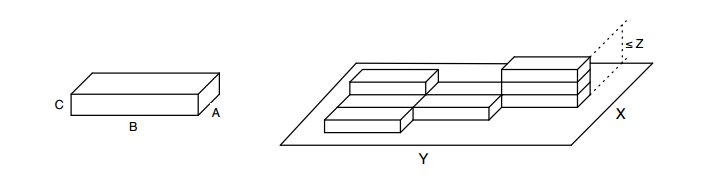
\includegraphics[scale=0.6]{problems/transporte/imagens/transporte.jpg}
\end{center}


Devido a limitações do guindaste utilizado, os contêineres só podem ser
carregados alinhados com o navio. Ou seja, os contêineres só podem ser colocados
sobre o navio de tal forma que a largura e o comprimento do contêiner estejam
paralelos à largura e ao comprimento do navio, respectivamente.

A SBC está com problemas para saber qual a quantidade máxima de contêineres que
podem ser colocados no navio e pede sua ajuda. Sua tarefa, neste problema, é
determinar quantos contêineres podem ser carregados no navio respeitando as
restrições acima.

\subsection*{Entrada}

A entrada contém vários casos de teste. Cada caso de teste consiste de duas
linhas. A primeira linha contém três inteiros $A$, $B$ e $C$ que representam as
dimensões dos contêineres, enquanto a segunda linha contém
outros três inteiros $X$, $Y$ e $Z$ que representam as dimensões do navio.

A entrada termina com fim-de-arquivo (EOF). As restrições são:

\begin{itemize}
    \item $1 \leq A, B, C, X, Y, Z \leq 10^6$
    \item É garantido que a maior resposta será menor ou igual a $10^6$
\end{itemize}

\subsection*{Saída}

Para cada caso de teste, seu programa deve imprimir apenas uma linha contendo um
inteiro que indica a quantidade máxima de contêineres que o navio consegue transportar.

\begin{table}[!h]
\centering
\begin{tabular}{|l|l|}
\hline
\begin{minipage}[t]{3in}
\textbf{Exemplo de entrada}
\begin{verbatim}
1 1 1
1 1 1
1 2 5
9 6 11
1 2 12
6 9 10
\end{verbatim}
\vspace{1mm}
\end{minipage}
&

\begin{minipage}[t]{3in}
\textbf{Exemplo de saída}
\begin{verbatim}
1
54
0
\end{verbatim}
\vspace{1mm}
\end{minipage} \\
\hline
\end{tabular}
\end{table}

\newpage
